\documentclass[aspectratio=169]{beamer}
\setbeamersize{text margin left=0mm,text margin right=0mm} 
\setbeamertemplate{navigation symbols}{}
\usepackage{fancyvrb}
\definecolor{MyBackground}{RGB}{247    245    231}
\setbeamercolor{background canvas}{bg=MyBackground}
\usepackage{graphicx} 
\usepackage{xcolor}
\usepackage[absolute,overlay]{textpos}
\usepackage{tikz}
\usetikzlibrary{lindenmayersystems}

\begin{document}
\begin{frame}
\begin{textblock*}{\linewidth}(3mm,5mm)
\fcolorbox{black}{white}{\begin{minipage}[t][0.46\linewidth][c]{0.45\linewidth}
\centering
\def\trianglewidth{2cm}%
\pgfdeclarelindenmayersystem{Sierpinski triangle}{
    \symbol{X}{\pgflsystemdrawforward}
    \symbol{Y}{\pgflsystemdrawforward}
    \rule{X -> X-Y+X+Y-X}
    \rule{Y -> YY}
}%
\foreach \level in {3,...,5}{%
\tikzset{
    l-system={step=\trianglewidth/(2^\level), 
    order=\level, angle=-120}
}%
\begin{tikzpicture}
    \fill [black] (0,0) -- ++(0:\trianglewidth) 
    -- ++(120:\trianglewidth) -- cycle;
    \draw [draw=none] (0,0) l-system
    [l-system={Sierpinski triangle, axiom=X},fill=white];
\end{tikzpicture}
}%
\end{minipage}
}%
\hspace{1mm}
\fcolorbox{black}{white}{\begin{minipage}[t][0.46\linewidth][c]{0.45\linewidth}
{\tiny\VerbatimInput{1.tex}}
\end{minipage}
}%
\end{textblock*}
\end{frame}

\begin{frame}
\begin{textblock*}{\linewidth}(3mm,5mm)
\fcolorbox{black}{white}{\begin{minipage}[t][0.46\linewidth][c]{0.45\linewidth}
\centering
\input{2}
\end{minipage}
}%
\hspace{1mm}
\fcolorbox{black}{white}{\begin{minipage}[t][0.46\linewidth][c]{0.45\linewidth}
{\tiny\VerbatimInput{2.tex}}
\end{minipage}
}%
\end{textblock*}
\end{frame}

\begin{frame}
\begin{textblock*}{\linewidth}(3mm,5mm)
\fcolorbox{black}{white}{\begin{minipage}[t][0.46\linewidth][c]{0.45\linewidth}
\centering
\pgfdeclarelindenmayersystem{Hilbert curve}{
  \symbol{X}{\pgflsystemdrawforward}
  \symbol{+}{\pgflsystemturnright}
  \symbol{-}{\pgflsystemturnleft}
  \rule{A -> +BX-AXA-XB+}
  \rule{B -> -AX+BXB+XA-}
}
\tikz\draw[lindenmayer system={Hilbert curve, axiom=A, 
  order=4, angle=90}]
  lindenmayer system;
\end{minipage}
}%
\hspace{1mm}
\fcolorbox{black}{white}{\begin{minipage}[t][0.46\linewidth][c]{0.45\linewidth}
{\tiny\VerbatimInput{3.tex}}
\end{minipage}
}%
\end{textblock*}
\end{frame}

\begin{frame}
\begin{textblock*}{\linewidth}(3mm,5mm)
\fcolorbox{black}{white}{\begin{minipage}[t][0.46\linewidth][c]{0.45\linewidth}
\centering
\tikz[rotate=65]\draw [gray!60!black] l-system
  [l-system={rule set={F -> F[+F]F[-F]}, axiom=F, order=4, angle=25,step=3pt}];
\end{minipage}
}%
\hspace{1mm}
\fcolorbox{black}{white}{\begin{minipage}[t][0.46\linewidth][c]{0.45\linewidth}
{\tiny\VerbatimInput{4.tex}}
\end{minipage}
}%
\end{textblock*}
\end{frame}

\begin{frame}
\begin{textblock*}{\linewidth}(3mm,5mm)
\fcolorbox{black}{white}{\begin{minipage}[t][0.46\linewidth][c]{0.45\linewidth}
\centering
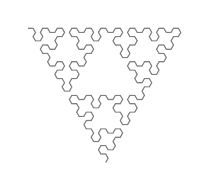
\begin{tikzpicture}[l-system={step=1.75pt, order=5, angle=60}]
  \pgfdeclarelindenmayersystem{ast}{
    \symbol{X}{\pgflsystemdrawforward}
    \symbol{Y}{\pgflsystemdrawforward}
    \rule{X -> Y-X-Y}
    \rule{Y -> X+Y+X}
  }
  \draw [gray] (3,2) l-system
    [l-system={ast, axiom=X, anchor=north east}];
\end{tikzpicture}
\end{minipage}
}%
\hspace{1mm}
\fcolorbox{black}{white}{\begin{minipage}[t][0.46\linewidth][c]{0.45\linewidth}
{\tiny\VerbatimInput{5.tex}}
\end{minipage}
}%
\end{textblock*}
\end{frame}

\begin{frame}
\begin{textblock*}{\linewidth}(3mm,5mm)
\fcolorbox{black}{white}{\begin{minipage}[t][0.46\linewidth][c]{0.45\linewidth}
\centering
\pgfdeclarelindenmayersystem{Koch curve}{
  \rule{F -> F-F++F-F}}
  \begin{tikzpicture}
\draw 
[l-system={Koch curve, step=2pt, angle=60, axiom=F++F++F, order=4}]
lindenmayer system -- cycle;
\end{tikzpicture}
\end{minipage}
}%
\hspace{1mm}
\fcolorbox{black}{white}{\begin{minipage}[t][0.46\linewidth][c]{0.45\linewidth}
{\tiny\VerbatimInput{6.tex}}
\end{minipage}
}%
\end{textblock*}
\end{frame}

\end{document}


1) Lavorando in un repo locale, fare git add, git commit, gitignore
https://github.com/github/gitignore

2) Lavorando in un repo locale, fare git checkout, git branch

3) Lavorando in un repo locale, fare git merge

4) Lavorando in un repo locale, visualizzare conflitti tra due branch

5) Lavorando in un repo locale, come tornare a un commit vecchio e come ammazzare gli ultimi uncommitted changes
https://github.blog/2015-06-08-how-to-undo-almost-anything-with-git/

6) Le stesse cose di prima, ma da un branch remoto
git push, git pull

7) Conflitti con branch remoto (Fare pull prima di push)

8) Pull request 